\documentclass{article}
\usepackage[utf8]{inputenc}
\usepackage{graphicx} % Required for inserting images
\usepackage{amsmath}

\title{Math equations using LaTeX}
\author{Debashish Chakraborty}
\date{February 2024}

\begin{document}
\maketitle

\section*{Introduction}
% To write a comment we use the percentage sign
Let's begin with a formula:

$$\textit{$e^{i\pi}+1=0$.}$$

\begin{itemize}
\item But we can also do,

$$e= \lim_{n\to\infty} \left(1+\frac{1}{n}\right)^n = \lim_{n\to\infty} \frac{n}{\sqrt[n]{n!}} $$

\item We can do another:

$$e = \sum_{n=0}^\infty \frac{1}{n!}$$

\item We can also use continued fractions:

$$e = 2+\frac{1}{1+\frac{1}{2+\frac{2}{3+\frac{3}{4+\ddots}}}}$$
\end{itemize}

\section*{More formulas}
\begin{enumerate}
\item Definite integral:
$$\int_a^bf(x)dx$$
\item Triple integral: 
$$\iiint f(x,y,z)dxdydz$$
\item Vector:
$$\vec{v} = <v_1.v_2,v_3>$$
\item Dot product:
$$\vec{v}\cdot\vec{w}$$
\item Matrix:
$$\begin{bmatrix}
1 & 2 & 3\\
4 & 5 & 6\\
\end{bmatrix}
$$
\end{enumerate}

%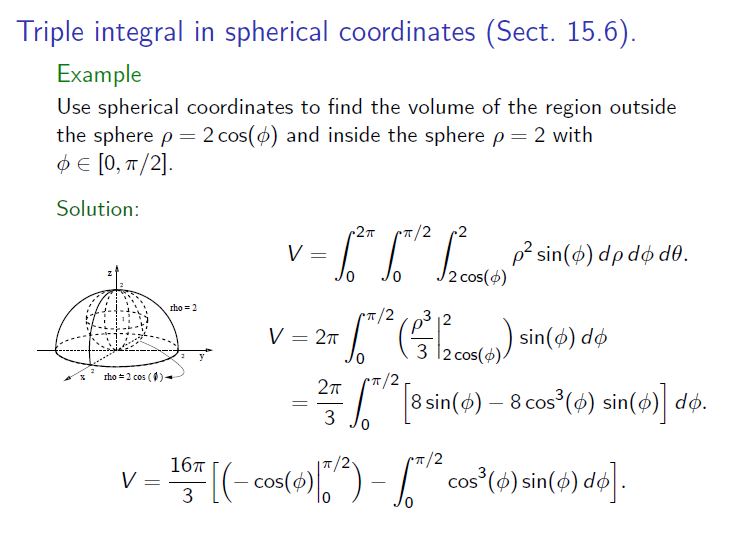
\includegraphics[scale=0.5]{integral.png}

\end{document}
